% Drawing 154/09-9 -- folder 154, batch 09, archive page 174 (PDF page 175).
% Transcription: dessins en couleur et au crayon sans texte : un disque rouge traversé de pseudo-droites rouges, bordé d'une couronne de pétales vert clair séparés par des coins vert foncé ; le même disque à moitié entouré, avec trois pétales au crayon, des coins bleus et vert foncé et, au bord, des numéros $1'$, $2'$, $3'$, $4'$, $5'$, $1$, $2$, $3$, $4$, $5$ ; un petit disque à trois pétales au crayon, un arc du bord fléché ; un disque traversé de trois droites rouges en triangle, un arc du bord bleu ; au crayon, une sphère coupée de grands cercles et deux polyèdres en perspective
% Kind: disk with a crown of light green petals; the same half-crowned; disks with arrangements; pencil sketches. Method 2 (schematic redraw from the facsimile). Status: partial.
% Notes: Colour and pencil drawings without text, read from the page view: a red disk crossed by red pseudolines, bordered by a crown of light green petals separated by dark green corners (16 petals drawn; the rim grey-blue); the same disk half crowned, with three pencil petals, blue and dark green corners and numbered rim points (not reproduced); a small disk with three pencil petals; a red disk with three chords; a pencil sphere and pencil polyhedra (a box and a hexagonal prism) drawn in outline. Strands schematic. Still differs from the facsimile: Colour and pencil drawings without text, read from the page view: a red disk crossed by red pseudolines, bordered by a crown of light green petals separated by dark green corners (16 petals drawn; the rim grey-blue); the same disk half crowned, with three pencil petals, blue and dark green corners and numbered rim points (not reproduced); a small disk with three pencil petals; a red disk with three chords; a pencil sphere and pencil polyhedra (a box and a hexagonal prism) drawn in outline. Strands schematic.
% Coordinates: 1 unit = 1 mm = 1/100 of the crop width (bbox in page fractions: [0.18, 0.085, 0.937, 0.502]).
% Redrawn by Claude (claude-opus-5-5), issue #73, 2026-11-07; not checked by a human; not compiled (no TeX in the session).
% Revised by Claude (claude-opus-5-5) 2026-11-09 (issue #128) after Michel's check: vertices snapped to exact intersections (drawn points on their lines, meeting ends on the stroke they meet, near-concurrent lines through one computed point, curve ends on their rim); labels at \small as in folder 80 batch 3. Status: partial.
% Rights: reproduces part of the work -- behind RENDER_TRANSCRIPTS, never published by itself.
\documentclass[tikz,border=3pt]{standalone}
\usepackage{amsmath,amssymb}
\usetikzlibrary{patterns,arrows.meta}
\tikzset{Or/.style={orange!90!black}, Ye/.style={yellow!80!orange}, Lg/.style={green!60!black!70}, Dg/.style={green!45!black}, Br/.style={brown!80!black}, Rd/.style={red!85!black}, Bl/.style={blue!70!black}, Gy/.style={black!40}, pencil/.style={black!45}, struck/.style={black!35}, mark/.style={circle,draw,inner sep=1.3pt}, pt/.style={circle,fill,inner sep=0.9pt}, opt/.style={circle,draw,fill=white,inner sep=1.1pt}}
\begin{document}
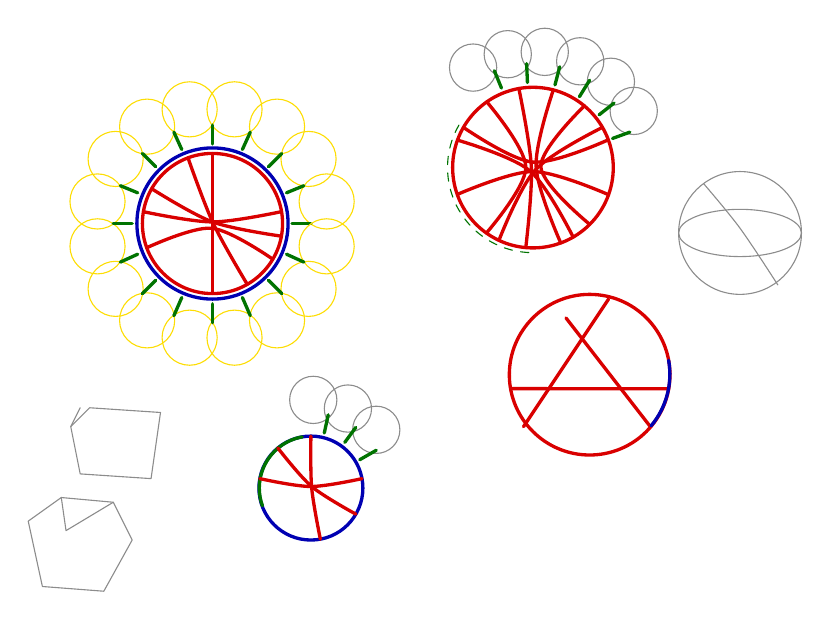
\begin{tikzpicture}[x=1mm,y=1mm,line cap=round,line join=round,font=\scriptsize]
\draw[Bl,very thick] (24.6,-29.3) circle[radius=9.6];
\draw[Rd,very thick] (24.6,-29.3) circle[radius=8.9];
\draw[Rd,very thick] plot[smooth, tension=0.55] coordinates {(24.6,-20.4) (24.6,-29.3) (24.6,-38.2)};
\draw[Rd,very thick] plot[smooth, tension=0.55] coordinates {(21.49,-20.96) (24.7,-29.3) (29.02,-37.03)};
\draw[Rd,very thick] plot[smooth, tension=0.55] coordinates {(15.83,-27.8) (24.6,-29.1) (33.37,-27.79)};
\draw[Rd,very thick] plot[smooth, tension=0.55] coordinates {(16.25,-32.38) (24.5,-29.9) (32.26,-33.83)};
\draw[Rd,very thick] plot[smooth, tension=0.55] coordinates {(16.87,-24.88) (24.6,-29.1) (33.35,-30.91)};
\draw[Ye] (39.1,-26.5) circle[radius=3.5];
\draw[Dg,very thick] (34.7,-29.3) -- (37.1,-29.3);
\draw[Ye] (36.8,-21.1) circle[radius=3.5];
\draw[Dg,very thick] (34,-25.4) -- (36.2,-24.5);
\draw[Ye] (32.8,-17) circle[radius=3.5];
\draw[Dg,very thick] (31.7,-22.1) -- (33.4,-20.4);
\draw[Ye] (27.4,-14.8) circle[radius=3.5];
\draw[Dg,very thick] (28.4,-19.9) -- (29.4,-17.7);
\draw[Ye] (21.7,-14.8) circle[radius=3.5];
\draw[Dg,very thick] (24.6,-19.2) -- (24.6,-16.8);
\draw[Ye] (16.3,-17) circle[radius=3.5];
\draw[Dg,very thick] (20.7,-19.9) -- (19.7,-17.7);
\draw[Ye] (12.3,-21.1) circle[radius=3.5];
\draw[Dg,very thick] (17.4,-22.1) -- (15.7,-20.4);
\draw[Ye] (10,-26.5) circle[radius=3.5];
\draw[Dg,very thick] (15.1,-25.4) -- (12.9,-24.5);
\draw[Ye] (10,-32.2) circle[radius=3.5];
\draw[Dg,very thick] (14.4,-29.3) -- (12,-29.3);
\draw[Ye] (12.3,-37.6) circle[radius=3.5];
\draw[Dg,very thick] (15.1,-33.2) -- (12.9,-34.2);
\draw[Ye] (16.3,-41.6) circle[radius=3.5];
\draw[Dg,very thick] (17.4,-36.5) -- (15.7,-38.2);
\draw[Ye] (21.7,-43.8) circle[radius=3.5];
\draw[Dg,very thick] (20.7,-38.7) -- (19.7,-41);
\draw[Ye] (27.4,-43.8) circle[radius=3.5];
\draw[Dg,very thick] (24.6,-39.5) -- (24.6,-41.9);
\draw[Ye] (32.8,-41.6) circle[radius=3.5];
\draw[Dg,very thick] (28.4,-38.7) -- (29.4,-41);
\draw[Ye] (36.8,-37.6) circle[radius=3.5];
\draw[Dg,very thick] (31.7,-36.5) -- (33.4,-38.2);
\draw[Ye] (39.1,-32.2) circle[radius=3.5];
\draw[Dg,very thick] (34,-33.2) -- (36.2,-34.2);
\draw[Rd,very thick] (65.3,-22.2) circle[radius=10.2];
\draw[Dg,dashed] (55.9,-16.8) arc[start angle=150, end angle=270, x radius=10.8, y radius=10.8];
\draw[Rd,very thick] plot[smooth, tension=0.55] coordinates {(63.51,-12.16) (65.1,-22.2) (64.39,-32.36)};
\draw[Rd,very thick] plot[smooth, tension=0.55] coordinates {(67.89,-12.33) (65.7,-22.1) (68.83,-31.77)};
\draw[Rd,very thick] plot[smooth, tension=0.55] coordinates {(59.44,-13.85) (64.4,-22.2) (59.39,-30.51)};
\draw[Rd,very thick] plot[smooth, tension=0.55] coordinates {(71.83,-14.36) (66.3,-22.1) (72.51,-29.41)};
\draw[Rd,very thick] plot[smooth, tension=0.55] coordinates {(56.47,-17.09) (65.3,-21.5) (74.87,-18.67)};
\draw[Rd,very thick] plot[smooth, tension=0.55] coordinates {(55.69,-25.61) (65.3,-22.7) (74.9,-25.64)};
\draw[Rd,very thick] plot[smooth, tension=0.55] coordinates {(74.13,-17.09) (65.6,-22.5) (60.98,-31.44)};
\draw[Rd,very thick] plot[smooth, tension=0.55] coordinates {(55.72,-18.71) (64.9,-22.6) (70.41,-31.03)};
\draw[pencil] (78.1,-15) circle[radius=3];
\draw[Dg,very thick] (75.4,-18.5) -- (77.6,-17.7);
\draw[pencil] (75.2,-11.3) circle[radius=3];
\draw[Dg,very thick] (73.7,-15.5) -- (75.6,-14);
\draw[pencil] (71.3,-8.7) circle[radius=3];
\draw[Dg,very thick] (71.2,-13.2) -- (72.5,-11.1);
\draw[pencil] (66.8,-7.5) circle[radius=3];
\draw[Dg,very thick] (68.1,-11.7) -- (68.7,-9.4);
\draw[pencil] (62.1,-7.8) circle[radius=3];
\draw[Dg,very thick] (64.6,-11.4) -- (64.5,-9);
\draw[pencil] (57.7,-9.5) circle[radius=3];
\draw[Dg,very thick] (61.3,-12.1) -- (60.4,-9.9);
\draw[Bl,very thick] (37.1,-62.9) circle[radius=6.6];
\draw[Dg,very thick] (36,-56.4) arc[start angle=100, end angle=200, x radius=6.6, y radius=6.6];
\draw[Rd,very thick] plot[smooth, tension=0.55] coordinates {(37.1,-56.3) (37.2,-62.9) (38.3,-69.39)};
\draw[Rd,very thick] plot[smooth, tension=0.55] coordinates {(30.61,-61.7) (37.1,-62.7) (43.59,-61.7)};
\draw[Rd,very thick] plot[smooth, tension=0.55] coordinates {(32.9,-57.81) (37.2,-62.7) (42.81,-66.21)};
\draw[pencil] (45.4,-55.5) circle[radius=3];
\draw[Dg,very thick] (43.3,-59.3) -- (45.4,-58.1);
\draw[pencil] (41.8,-52.8) circle[radius=3];
\draw[Dg,very thick] (41.4,-57.1) -- (42.8,-55.2);
\draw[pencil] (37.4,-51.7) circle[radius=3];
\draw[Dg,very thick] (38.8,-55.9) -- (39.3,-53.6);
\draw[Rd,very thick] (72.5,-48.5) circle[radius=10.2];
\draw[Rd,very thick] (64.1,-55.1) -- (74.9,-38.9);
\draw[Rd,very thick] (69.5,-41.3) -- (80.24,-55.14);
\draw[Rd,very thick] (62.46,-50.27) -- (82.54,-50.29);
\draw[Bl,very thick] (80.3,-55) arc[start angle=-40, end angle=10, x radius=10.2, y radius=10.2];
\draw[pencil] (91.6,-30.5) circle[radius=7.8];
\draw[pencil] (91.6,-30.5) ellipse[x radius=7.8, y radius=3];
\draw[pencil] plot[smooth, tension=0.55] coordinates {(86.97,-24.23) (91.6,-29.9) (96.4,-37.1)};
\draw[pencil] (6.6,-55.1) -- (7.8,-61.1) -- (16.8,-61.7) -- (18,-53.3) -- (9,-52.7) -- cycle;
\draw[pencil] (6.6,-55.1) -- (7.8,-52.7);
\draw[pencil] (1.2,-67.1) -- (5.4,-64.1) -- (12,-64.7) -- (14.4,-69.5) -- (10.8,-76) -- (3,-75.4) -- cycle;
\draw[pencil] (5.4,-64.1) -- (6,-68.3) -- (12,-64.7);
\end{tikzpicture}
\end{document}
